\section{Population Generation}

After the terrain has been generated, the PopulationGenerator provides the user with a tool to mark areas on the terrain where they want cities to be placed. 
When one or more markers are placed, they will remain in their designated positions until interacted with by the user, or when the user presses the Generate Roads button.

A placed city marker can be interacted with by hovering over it, which will turn it red.
Clicking on it will make it yellow, which shows that it is selected. 

\begin{figure}[h!]
  \centering

  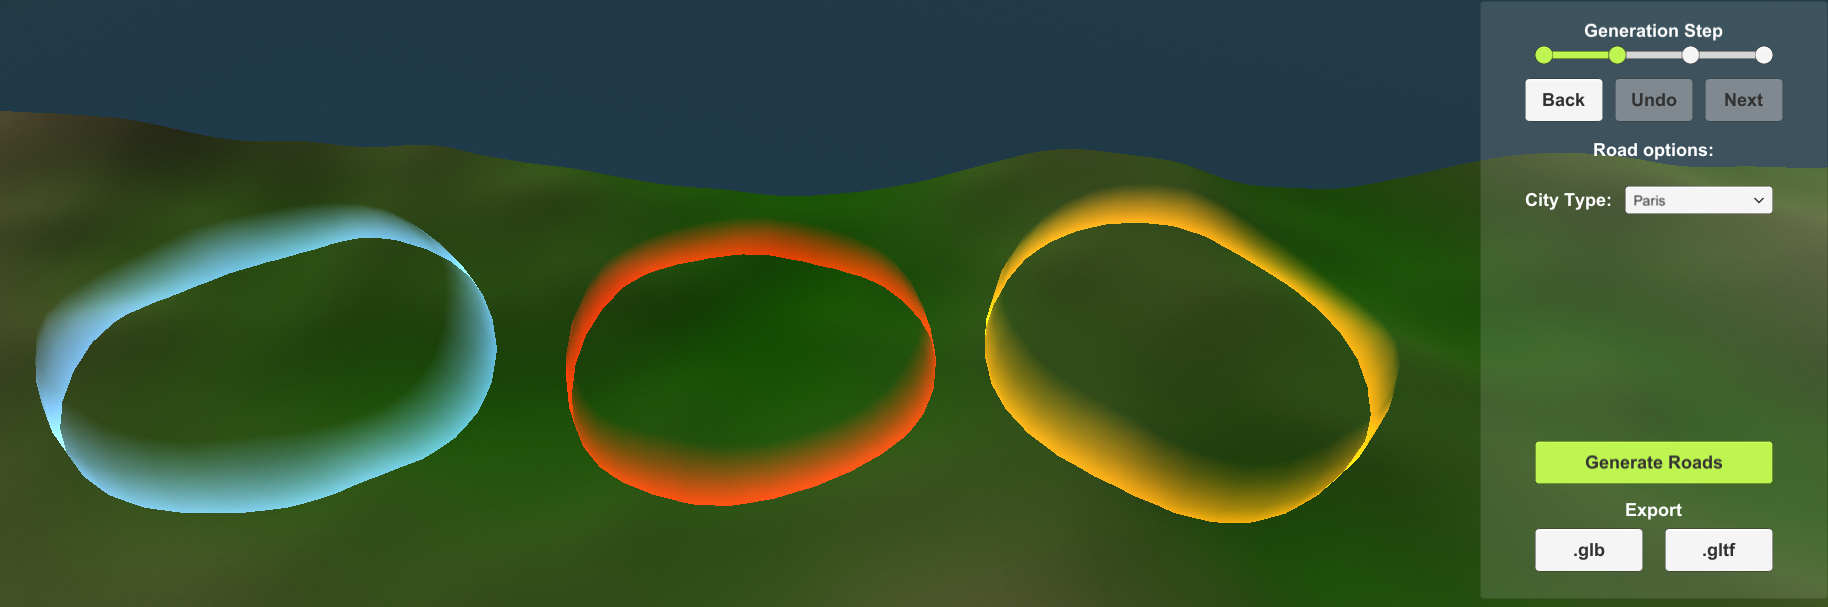
\includegraphics[width=0.8\textwidth]{figure/citymarkers.png}
  \caption{The city marker tool visuals. }

  \label{fig:citymarkers}
\end{figure}

The selected city marker has multiple options:
\begin{easylist}
  @ Clicking again and dragging will allow the user to freely reposition the marker.
  @ Scrolling up and down will increase and decrease the effective radius.
  @ Deleting it can be done by pressing the Delete key on the keyboard when selected.
\end{easylist}


Population generation begins after pressing the generate roads button.
Before the roads are generated, a population density map is generated which covers the entire terrain.
Then, the city marker amplifiers add density to the base noise generated in the spots where it was placed.

When the population generator is finished, the road generation begins.
Its roads and highways will tend towards densely populated areas, and the size of buildings will vary depending on how intense the density is.
